% Figure 1: Rosetta interface energies
\begin{figure}[htbp]
\centering
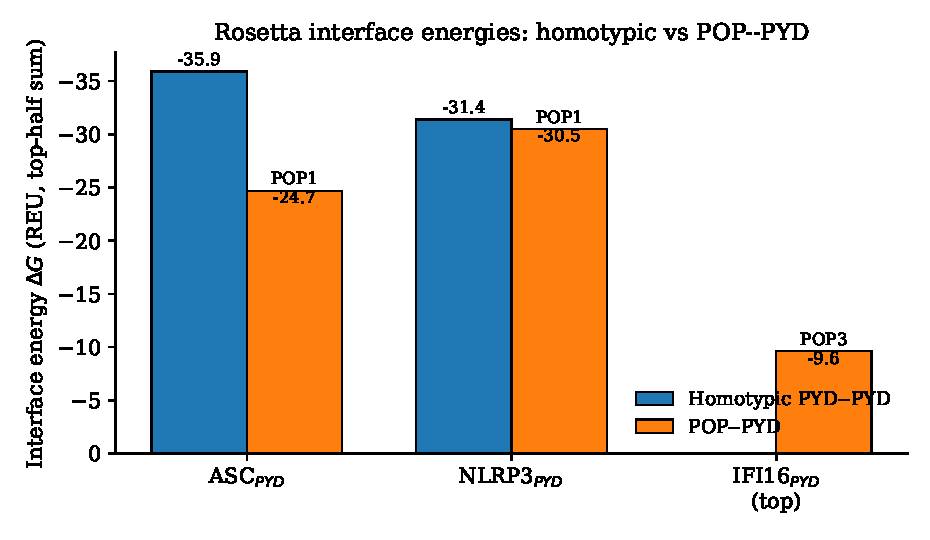
\includegraphics[width=0.78\textwidth]{figures/fig_rosetta_dg.pdf}
\caption{Rosetta InterfaceAnalyzer energies ($\Delta G$, Rosetta Energy Units)
for the top-half interfaces of homotypic PYD--PYD filaments and POP--PYD
substitutions. ASC$_{PYD}$--ASC$_{PYD}$ reaches $-35.9$~REU while POP1--ASC$_{PYD}$
is only $-24.7$~REU; POP1--NLRP3$_{PYD}$ ($-30.5$~REU) is nearly isoenergetic
with NLRP3$_{PYD}$--NLRP3$_{PYD}$ ($-31.4$~REU); POP3--IFI16$_{PYD}$ (top
half, $-9.6$~REU) is the strongest POP--IFI16 interaction.}
\label{fig:rosetta_dg}
\end{figure}

% Figure 2: Honeycomb schematic
\begin{figure}[htbp]
\centering
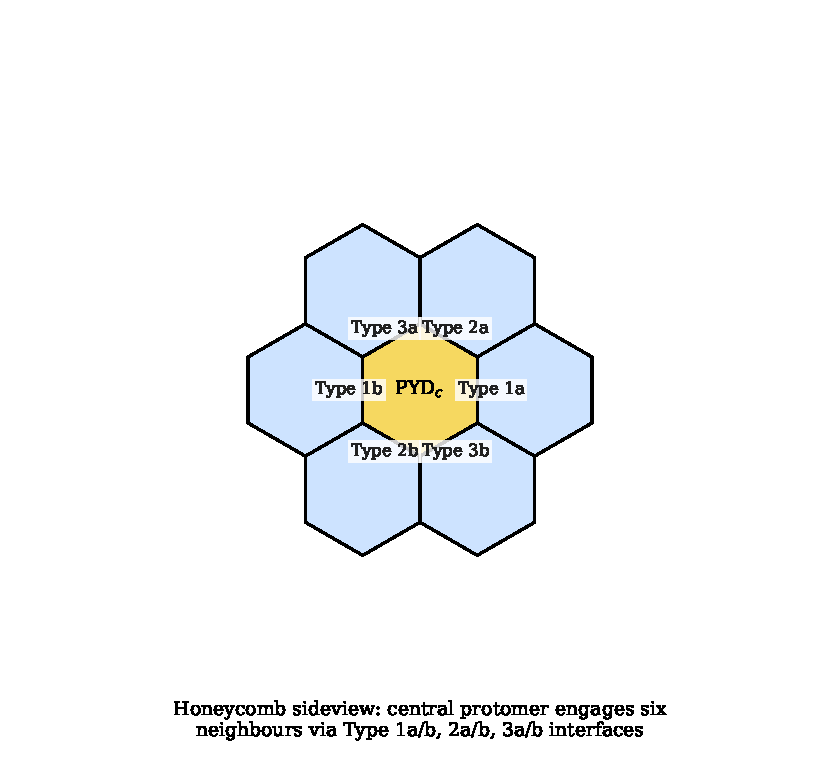
\includegraphics[width=0.55\textwidth]{figures/fig_honeycomb_schematic.pdf}
\caption{Honeycomb sideview strategy used for Rosetta interface analysis. The
central PYD protomer engages six neighbours through Type 1a/1b, Type 2a/2b
and Type 3a/3b interfaces, which together define the interfaces probed in all
homotypic and POP--PYD calculations.}
\label{fig:honeycomb}
\end{figure}

% Figure 3: Cellular POP1 suppression
\begin{figure}[htbp]
\centering
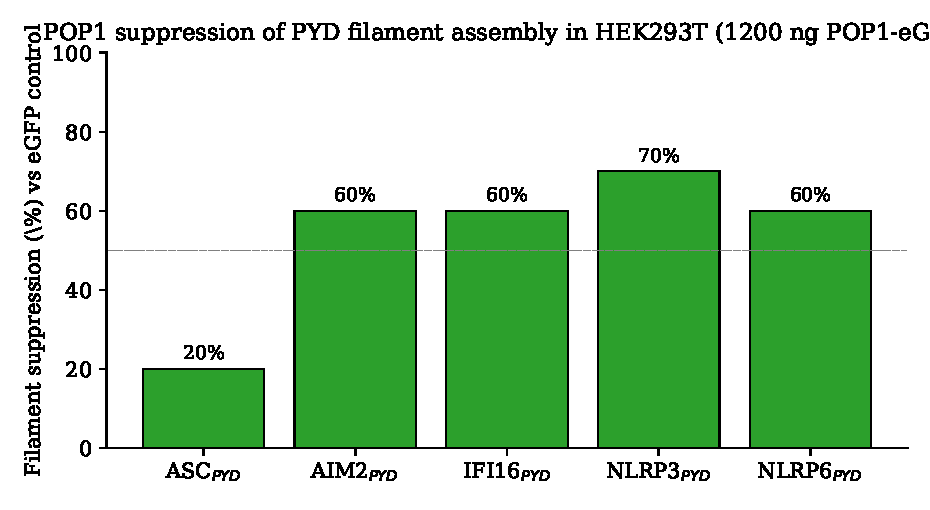
\includegraphics[width=0.78\textwidth]{figures/fig_pop1_suppression.pdf}
\caption{Cellular suppression of PYD filament assembly by 1200~ng POP1-eGFP
in HEK293T cells co-transfected with 300~ng of the indicated mCherry-tagged
PYD. POP1 is a weak inhibitor of ASC$_{PYD}$ ($\sim$20\% suppression) but
suppresses upstream receptor PYDs by 60--70\%.}
\label{fig:pop1_suppression}
\end{figure}

% Figure 4: FRET concentration ranges
\begin{figure}[htbp]
\centering
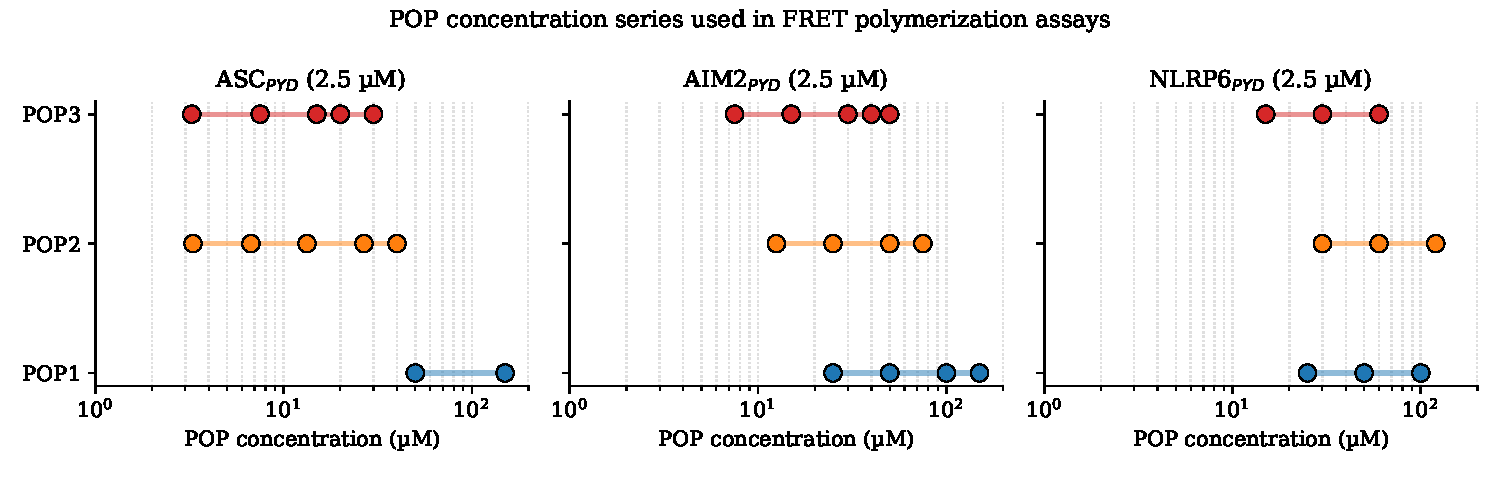
\includegraphics[width=\textwidth]{figures/fig_fret_concentrations.pdf}
\caption{POP concentration series used in FRET-based polymerization assays
against ASC$_{PYD}$, AIM2$_{PYD}$ and NLRP6$_{PYD}$ (each at 2.5~\textmu M).
POP1 is tested up to 150~\textmu M against ASC$_{PYD}$ and AIM2$_{PYD}$
and up to 100~\textmu M against NLRP6$_{PYD}$; POP2 and POP3 operate at
lower absolute concentrations.}
\label{fig:fret_concs}
\end{figure}

% Figure 5: Revised model schematic
\begin{figure}[htbp]
\centering
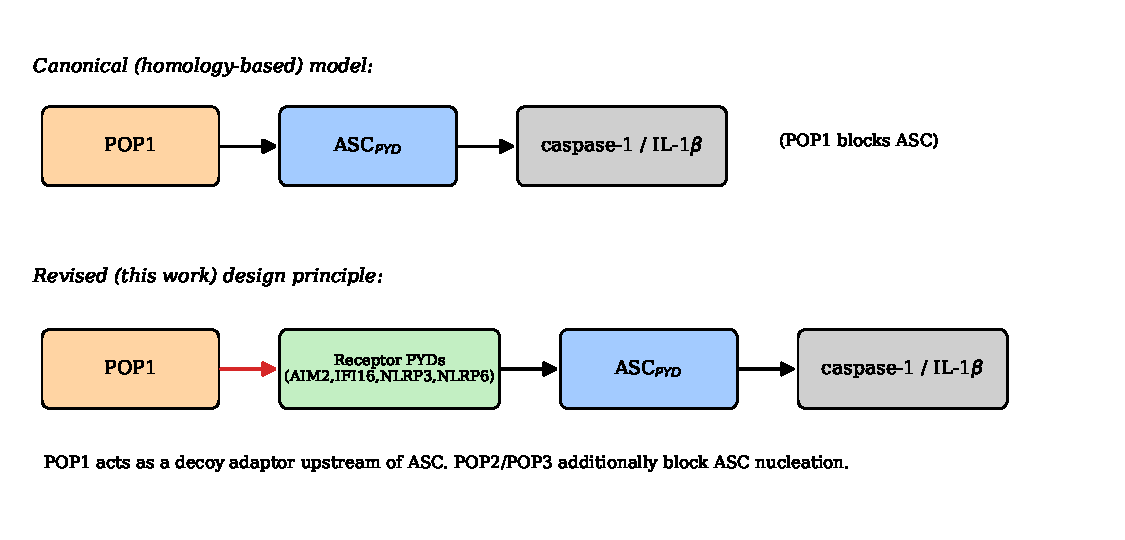
\includegraphics[width=0.95\textwidth]{figures/fig_model_schematic.pdf}
\caption{Canonical versus revised model of POP1 function. Sequence-homology
based models placed POP1 as a direct ASC inhibitor (top). Our combined
Rosetta, cellular, and biochemical data instead indicate that POP1 acts as
a decoy adaptor that throttles upstream receptor PYDs, while POP2 and POP3
additionally block ASC nucleation (bottom).}
\label{fig:model}
\end{figure}
